\documentclass{article}
\usepackage[margin=.5in]{geometry}
\usepackage{amsfonts}
\usepackage{amssymb}
\usepackage{amsmath}
\usepackage{graphicx}
\usepackage{algorithm}
\usepackage{algpseudocode}

\begin{document}
\begin{center}
{\huge \bf CS 6350 Midterm Review}
\end{center}


\hspace{-1.5em}{\large \bf General Supervised Learning}
\begin{itemize}
\item Supervised learning, instance spaces, label spaces, concept and hypothesis spaces
	\begin{itemize}
	\item {\bf Supervised learning:} 
		\begin{itemize}
		\item Given some training examples in the form $\left< x,f(x)\right>$, with $f$ being unknown
		\item Typically, the input $x$ is represented in the {\em feature space}, for example $x\in \{0,1\}^{n}\text{ or }x\in \mathbb{R}^{n}$
		\item For a training example $x$, the value of $f(x)$ is called its {\em label}
		\item \underline{Goal:} Find a good approximation for $f$. Aimes to decide: an instance space, determine the instance space's label space, the necessary hypothesis space to do so, and evaluate uncertainty.
		\end{itemize}
	\item {\bf Instance spaces:} The set of the examples and features that are going to be looked at. Often elements of the instance space are \textbf{feature vectors}. 
	\item {\bf Label spaces:} The total set of possible labels that each instance can have
	\item {\bf Concept and Hypothesis spaces:}
		\begin{itemize}
		\item {\bf Hypothesis space:} Set of functions that the learning algorithm is going to be searching over. Categorises a certain class with specific constraints and attributes.
		\item {\bf Concept space:} Set of functions from which the classifier originates. Concept space is a set of functions from which the true classifier (also known as oracle) originates. The concept space contains the target classifier that is hidden from us. 
		\end{itemize}
	\end{itemize}
\item Understanding why we need to restrict hypothesis spaces
	\begin{itemize}
	\item Choose a hypothesis space that is smaller than the space of all functions. The functions that are choosen are done by either prior knowledge or by guessing. It also needs to be flexible enough to work with the data and not too small that nothing agrees with it.
	\item For example, in the case of boolean functions, can do only {\em simple conjunctions}, pick {\em m-of-n rules} where you pick a set of $n$ variables, of which at least $m$ need to be true, linear functions, etc.
	\item At times we are able to ``count functions'' within our restricted hypothesis space. In the case of booleans we have a total of $2^{2^n}$ functions. We can place tighter bounds on the order of our hypothesis space when considering only simple conjunctions or m-of-n rules.
	\end{itemize}
\item General issues in supervised learning: hypothesis spaces, representation (i.e. features), learning algorithms
	\begin{itemize}
	\item {\bf Hypothesis spaces:} If the hypothesis space is too large, then learning can not be done because there are too many functions to search over. Therefore, to be able to learn, the hypothesis space must be restricted to a smaller subset so that it is possible to learn.
	\item {\bf Representation/features:} Need features that represent the data well. Features that aren't present in a lot of the data {\em or} have too common of a value are not good features.
	\item {\bf Learning algorithms:} The right learning algorithm needs to be choosen such that it can learn from the data well and not be excessive in resource usage. Also you want an algorithm that doesn't overfit the data and has a high success rate.
	\end{itemize}
\end{itemize}


\hspace{-1.5em}{\large \bf Decision Trees}
\begin{itemize}
\item What is a decision tree? What can they represent?
	\begin{itemize}
	\item {\bf Decision tree:} A {\em hierarchical data structure} that represents data using a divide-and-conquor strategy. It can be used as a hypothesis class for non-parametric classification or regression. 

	\underline{General Idea:} Given a collection of examples, learn a decision tree that represents it.
	\item Decision trees are a family of classifiers for instances that are represented by feature vectors (i.e. vectors of attributes)
	\item Decision trees are built based on a {\em greedy hueristic}
	\item {\em Nodes} are tests for feature vectors
	\item There is one {\em branch} for every value that the feature can take
	\item {\em Leaves} of the tree specify the class labels
	\item Decision trees {\em can represent} all boolean functions. Decision trees are often used with discretely labeled instances. 
	\end{itemize}
\item How to predict with a decision tree
	\begin{itemize}
	\item At the root node, you're given a test, you then follow the branch for the correct answer for that one node. Decision trees need not be binary!
	\end{itemize}
\item Expressivity, counting the number of decision trees
	\begin{itemize}
	\item {\bf Expressivity:} 
	\end{itemize}
\item Dealing with continuous features
	\begin{itemize}
	\item You would have ranges of values that fall in to each node. For example:
	\begin{center}
	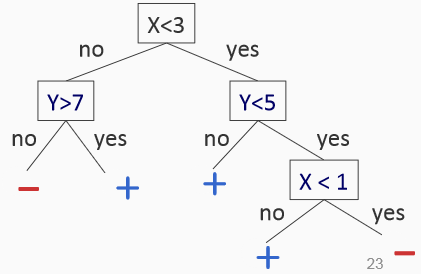
\includegraphics[width=.3\textwidth]{continuous.png}
	\end{center}
	\item If features are continuous, say irrational numbers, we must apply a discrete feature representation for our data. 
	\end{itemize}
\item Learning Algorithm: The ID3 algorithm entropy information gain
	\begin{itemize}
	\item The ID3 Algorithm is based on the {\em entropy} of each attribute

	{\bf ID3}($S$, {\tt Attributes}, {\tt Label}):

		\begin{enumerate}
		\item {\bf If} all examples have the same label:
		
		\hspace{2em}{\bf Return} a single node tree with the label
		\item {\bf Else:}
			\begin{enumerate}
			\item Create a \verb~Root Node~ for the tree
			\item \verb~A~ = attribute in \verb~Attributes~ that {\em \underline{best}} classifies $S$
			\item {\bf for each} possible value $\nu$ that \verb~A~ can take:
				\begin{enumerate}
				\item Add a new tree branch corresponding to \verb~A~ $=\nu$
				\item Let $S_{\nu}$ be the subset of examples in $S$ with \verb~A~ $ =\nu$
				\item {\bf If} $S_{\nu}\in\varnothing$:
				
				\hspace{1em}Add leaf node with the common value of \verb~Label~ in $S$
	
				{\bf Else}:

				\hspace{1em} Below this branch add the subtree \verb~ID3~($S\nu$,{\tt Attributes}$-\{${\tt A}$\}$,{\tt Label})
				\end{enumerate}
			\item {\bf Return} \verb~Root Node~
			\end{enumerate}
		\end{enumerate}
	\item {\bf Entropy and Information Gain:}
		\begin{itemize}
		\item {\em Entropy} is the set of examples $S$ with respect to binary classification is
		\begin{align*}
		Entropy(S) &= H(S) = -p_{+}\log_{2}\left(p_{+}\right)-p_{-}\log_{2}\left(p_{-}\right)\quad \left\{\begin{matrix}
p_{+}\text{ is the porportion of positive examples} \\\ \\
p_{-}\text{ is the proportion of negative examples}
\end{matrix}\right.\\
		Gain(S,A) &= Entropy(S) - \sum_{\nu\in\text{Values}}\frac{\left|S_{\nu}\right|}{\left| S\right|}Entropy\left(S_{\nu}\right)\\
		&S_{\nu}:  \ \ \text{The subset of examples where the value of attribute $A$ is set to value $\nu$}
		\end{align*}
		\end{itemize}
	\item The root attribute that should be choosen is the attribute with the highest information gain
	\item Information gain allows us to split over given examples so they are \textit{relatively pure in one label}. By splitting such that there is a reduction in entropy there is less uncertainty when labeling and a more structured partitioning of labels. 
	\end{itemize}
\item Overfitting (applicable not just to decision trees) and how to deal with it when training decision trees
	\begin{itemize}
	\item Consider some arbitrary function in the hypothesis space $h'$. With data coming from proability distribution $D$ a classifier $h$ can be considered overfit if :
	\begin{itemize}
	\item $error_{train}(h) ~<~error_{train}(h')$
	\item $error_D(h) ~ > ~ error_D(h')$
	\end{itemize}
	\item The learning algorithm fits the noise in the data. Irrelevant attribuytes or noisy examples influence the choice of the hypothesis
	\item May lead to poor performance on future examples
	\item Decision trees are notorous for overfitting, so the solution to this is to favor simpler (shorter) hypotheses as fewer shorter trees are less likely to fit better by coicidence
	\item \textit{Held-out-set} method is means to avoid over fitting by first setting a random sample of the training data aside then at every layer when building the decision tree test the current tree's performance on the held out set, if the performance drops stop growing the tree. The restricted height in theory should aide to avoid over fitting. This can be considered as pruning the tree greedily with a bottom up approach. 
	\end{itemize}
\item Dealing with missing features
	\begin{itemize}
	\item Using the most common value oif the attribute in the data
	\item Using the most common value of the attribute among all examples with the same output
	\item Using fractional counts of all the attributes and stochastically choosing a labeling when deciding with probaility equal to the fractional count.
	\item {\em Test time}: Use the same method
	\end{itemize}
\item When to use decision trees
	\begin{itemize}
	\item Binary classifications? Small hypothesis spaces?
	\end{itemize}
\end{itemize}


\hspace{-1.5em}{\large \bf Nearest Neighbors}
\begin{itemize}
\item Instance based learning. How to predict? Importance of representation
	\begin{itemize}
	\item Training examples are vectors $\mathbf{x}_{i}$ associated with a label $y_{i}$
	\item Since instance based, or ``memory based'' nearest neighbor is an expensive approach. 
	\item {\em Learning}: Just store all the training examples
	\item {\em Prediction}: For a new example $\mathbf{x}$, find the training example $\mathbf{x}_{i}$ that is {\em closest} to $\mathbf{x}$ and predict the label of $\mathbf{x}$ with the label $y_{i}$ associated with $\mathbf{x}_{i}$.
	\begin{itemize}
		\item {\em Classification}: Every neighbor votes on the label. Predict the most frequent label among the neighbors.
		\item {\em Regression}: Predict the mean value
	\end{itemize}
	\end{itemize}
\item Different definitions of distance
	\begin{itemize}
	\item Euclidean Distance
	\begin{align*}
	\left|\left| \mathbf{x}_{1} - \mathbf{x}_{2}\right|\right|_{2} = \sqrt{\sum_{i=1}^{n}\left(\mathbf{x}_{1,i}-\mathbf{x}_{2,i}\right)^{2}}
	\end{align*}
	\item Manhattan Distance
	\begin{align*}
	\left|\left| \mathbf{x}_{1} - \mathbf{x}_{2}\right|\right|_{1} = \sum_{i=1}^{n}\left|\mathbf{x}_{1,i}-\mathbf{x}_{2,i}\right|
	\end{align*}
	\item $L_{p}$-Norm
	\begin{align*}
	\left|\left| \mathbf{x}_{1} - \mathbf{x}_{2}\right|\right|_{p} = \left( \sum_{i=1}^{n}\left|\mathbf{x}_{1,i}-\mathbf{x}_{2,i} \right|^{p} \right)^{\frac{1}{p}}
	\end{align*}
	\end{itemize}
\item Dealing with symbolic features
	\begin{itemize}
	\item words. If the data under question is not real valued a common approach is to use \textit{the hamming distance}
	\end{itemize}
\item Choosing $k$ for $k$-NN
	\begin{itemize}
	\item $k$ must be odd to break ties
	\end{itemize}
\item Practical aspects: Feature normalization could be important
	\begin{itemize}
	\item Often, good idea to center the features to make them zero mean and unit standard deviation
	\item Because different features could have different scales (weight, height, etc); but the distance weights them equally
	\end{itemize}
\item Advantages and disadvantages
	\begin{itemize}
	\item {\bf Advantages:}
		\begin{itemize}
		\item Training is {\em very fast} since it's just adding labeled instances to a list
		\item Can learn very {\em complex functions}
		\item Always have the training data, so something can be done later if wanted
		\end{itemize}
	\item {\bf Disadvantages:}
		\begin{itemize}
		\item Needs a lot of storage
		\item Prediction can be slow as it has to check every instance, natively $\mathcal{O}(dN)$ for $N$ training examples and $d$ dimensions.
		\item Nearest neighbors are fooled by irrelevant attributes
		\end{itemize}
	\end{itemize}
\item Voronoi diagrams
	\begin{itemize}
	\item Voronoi diagrams map the region in question into colors for those regions that are closest to certain labels. This makes it easier for testing the test set as it can simply be put on the map and the color that it is in can be checked against the label.
	\begin{center}
	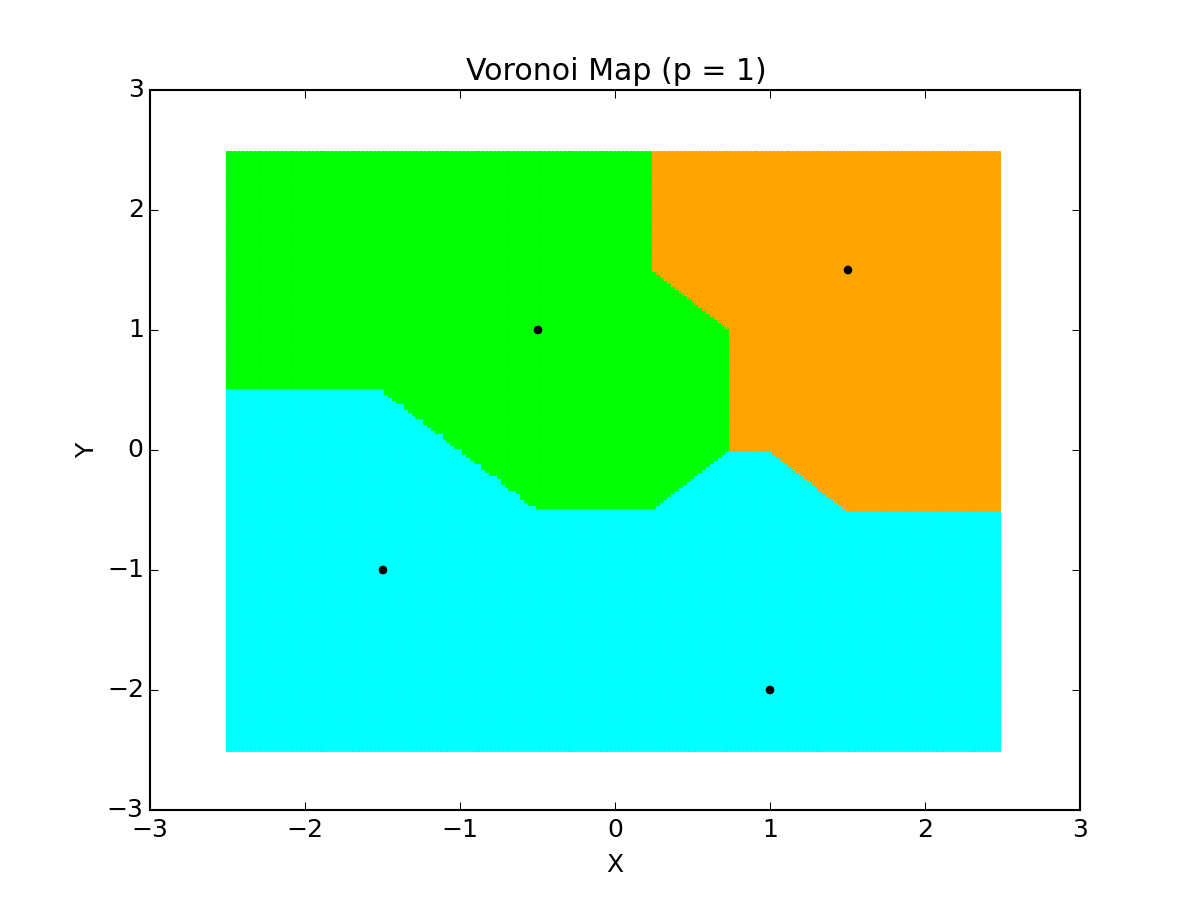
\includegraphics[width=.5\textwidth]{VoronoiMap_a1.png}\end{center}
	\end{itemize}

\item Curse of dimensionality (applicable beyond nearest neighbor algorithms)
	\begin{itemize}
	\item Methods that work with low dimensional spaces may fail in high dimensions
	\item What might be intuitive for 2 or 3 dimensions does not always apply to higher dimensional spaces
	\item {\em For Example:} If there is 1000 dimensional feature vectors, but only 10 are relevant, than the distances will be dominated by the large number of irrelevant features.
	\item For higher dimensions the sense of distance becomes abscured. For example when considering the amount of empty space between a sphere encased in a cube for higher dimensions the amount of space becomes unintuitively large. Mose volume is found on the boarder of the cube and as a result the sphere seems to approach zero and the amount of empty space grows rapidly. 
	\end{itemize}
\end{itemize}

\hspace{-1.5em}{\large \bf Linear Classifiers}
\begin{itemize}
\item What are they? Why are they interesting?
	\begin{itemize}
	\item Input is an $n$ dimensional vector $\mathbf{x}$, with the output being a label $y\in \{-1,1\}$
	\item {\em Linear Threshold Units} classify an example $\mathbf{x}$ using parameters $\mathbf{w}$ and $b$ according to the following classification rule
		\begin{itemize}
		\item Output = sign$(\mathbf{w}^{T}\mathbf{x} + b)$
		\item $\mathbf{w}^{T}\mathbf{x} + b \geq 0 \Rightarrow \text{predict } y = 1$
		\item $\mathbf{w}^{T}\mathbf{x} + b < 0 \Rightarrow \text{predict } y = -1$
		\end{itemize}
	\end{itemize}
\item What can they express? What can they not express?
	\begin{itemize}
	\item Expressive hypothesis class
		\begin{itemize}
		\item Many functions are linear
		\item Often a good guess for a hypothesis space
		\item Some functions are not linear (i.e. \verb~XOR~, non-trivial boolean functions)
		\item However there are ways tof making them linear in a higher dimensional feature space
		\end{itemize}

	\end{itemize}
\item Geometry
	\begin{itemize}
	\item We can view the linear classifier as defining a {\em hyperplane} seperating instances in the answer space. 
	\item {\em Bias term} is needed because if $b$ is zero, then restricting the learner only to hyperplanes that go through the origin which may not be expressive enough
	\end{itemize}
\item Feature expansion to predict a broader set of functions
	\begin{itemize}
	\item {\em Forced Linearity} allows us to linearly classify non-linear data. For example we can take data to a higher dimension and perform linear classification in the raised dimension e.g. our instance space $x$ can be brought paired with a polynomial making our instance space $(x, x^2)$
	\end{itemize}
	\item Gradient Descent 
	\begin{itemize}
	\item Goal is to predict a real valued output using a feature representation of the input. We assume the output is a linear function of the inputs. 
	\item Learning is done by minimizing the total cost or loss function. Many algorithms in machine learning (perceptron ect...) follow this paradigm with different loss functions and different hypothesis space. 
	\item Gradient decent uses the bellow loss function
	\begin{itemize}
	\item $J(\mathbf{w}) = \frac{1}{2}\sum_{i=1}^{m}(y_i - \mathbf{w}^T\mathbf{x_i})^2$
	\end{itemize}
	\end{itemize}
\end{itemize}

\hspace{-1.5em}{\large \bf Mistake Bound Learning}
\begin{itemize}
\item One way of asking how god is your classifier
	\begin{itemize}
	\item words
	\end{itemize}
\item The general structure of an online learning algorithm
	\begin{itemize}
	\item words
	\end{itemize}
\item Goal: Counting Mistakes. What is a mistake bound algorithm
	\begin{itemize}
	\item a mistake bound, or error driven, algorithm only makes updates when a prediction is incorrect. The weight vector is only altered in the case a mistake is made. 
	\item mistake bound algorithm is a algorithm that will acheive a desired result after a reasonable amount of corrections due to mistakes. 
	\item The Perceptron Convergence Theorem states that, If there exists a set of weights that are amenable to treatment with Perceptron (i.e., the data is linearly separable), then the Perceptron learning algorithm will converge
	\end{itemize}
\item Halving algorithm
	\begin{itemize}
	\item words
	\end{itemize}
\item Perceptron algorithm, geometry of the update, margin, Novikoff's theorem, variants
	\begin{itemize}
	\item The number of mistakes made by the perceptron algorithm is bound by the dimensionality R and the margin $\gamma$. $\gamma$ defines the seperability of the data and is defined as the distance to the two nearest points in the positive and negative groupings of the instance space. The total number of mistakes is defined by $(\frac{R}{n})^2$. For booleans $R^2$ = n since the $L^2$ norm of an n dimenstional vector is $\sqrt{n}$.
	\item \textbf{Novikoff's Theorem} Percoptron requires a training set $T=\{ (x_1,y_1),(x_2,y_2),...,(x_i,y_i)\}$ and weight vectors $\mathbf{w}$ and unit vector \textbf{u}, i.e. $||\mathbf{u}|| = 1$. We can safely assume that our data bound by some sphere in $\mathbb{R}^n$, $||\mathbf{x}|| \leq R$ for $R\in \mathbb{R}^n$. Given that $T$ is linearly seperable there is some margin value $\gamma \in \mathbb{R}$ which represents the distance to the nearest point in $T$ to our weight vector: $\mathbf{u}^T\mathbf{w} \geq \gamma$. We can also assume our first weight vector is a zero vector, i.e. $||\mathbf{w_o}|| = 0. $Using the above we prove the mistake bound:\\
	\begin{center}
	First we exploit the fact that the weights are seperated by some margin value. $\mathbf{u^T}\mathbf{w_t} \geq \gamma$\\
	$\mathbf{u^T}\mathbf{w_{t+1}} \geq \mathbf{u^T}\mathbf{w_t} + y_i\mathbf{u^T}\mathbf{x_i}$ by the definition of a weight update.\\
	$\geq \mathbf{u^T}\mathbf{w_t} + \gamma $\\
	By induction down to $t=0$, and recall $w_o$ is the zero vector, we get\\
	$\mathbf{u^T}\mathbf{w_t} \geq \gamma$\\
	Now we use the fact the weights are bound. $||\mathbf{w_t}||^2 \leq tR^2$ \\
	$||\mathbf{w_{t+1}}||^2 = ||\mathbf{w_t} +y_i\mathbf{x_i}||^2 = ||\mathbf{w_t}||^2 + 2y_i\mathbf{w_{i}^{T}}\mathbf{x_i} + ||\mathbf{x_i}||^2$\\
	$\leq ||\mathbf{w_t}||^2 + R^2$\\
	Again through induction and the zero initial weight vector\\
	$||\mathbf{w_t}||^2 \leq R^2$\\
	We combine our two results\\
	$R\sqrt{t} \geq ||\mathbf{w_t}|| \geq \mathbf{u^Tw_t}$ The second inequality by cauchy schwartz.
	$\geq t\gamma$\\
	$t\leq (\frac{R}{\gamma})^2$
	
	
	\end{center}
	\item \textbf{Geometry} For a perceptron, the decision bound- ary is precisely where the sign of the activation, a, changes from −1 to +1. In other words, it is the set of points x that achieve zero ac- tivation. The points that are not clearly positive nor negative. For simplicity, we’ll first consider the case where there is no “bias” term (or, equivalently, the bias is zero). Formally, the decision boundary B is:\\
	\\$x:\sum_{d}w_dx_d = 0$\\
	\\The sum is the dot product between the weight vector and x. This  dot product is zero if the two vectors are perpendicular. The boundry is the perpendicular plane to w.
	\item \textbf{margin} Formally, given a data set D, a weight vector w and bias b, the margin of w, b on D is defined as:\\
	\\$margin(D,w,b) = min_{(x,y)\in D}y(w\cdot x + b)$ if w seperates D, $-\infty$ oherwise\\
	\\The margin on a data set is the largest obtainable margin, i.e. the supremum of the above.
	\end{itemize}
\item Winnow algorithm, mistake bound, balanced winnow
	\begin{itemize}
	\item Mistake bound of the winnow algorithm for k-disjunctions is $O(klogn)$
	\item to describe OR of r variables where r << n  takes O(rlog n) bits.
	\item Winnow \textbf{mistake bound} is O(r log n)
	\item Winnow learns the class of disjunctions in at most $2+3r(1+logn)$ mistakes
	\item the margin is $\gamma = \alpha / L_1 (w^*)L_{\infty}(X))$ with bound $O((1/(\gamma^{2}*logn)))$ \textbf{??}
	\end{itemize}
\item Perceptron vs. Winnow
	\begin{itemize}
	\item The perceptron algorithm does addative updates. The Winnow algorithm does multiplicative. The perceptron mistake bound for k-disjunction is $O(n)$. The winnow for k-disjunctions is $O(klogn)$. Proof?
	\item Use Winnow for multiplicative algorithms: If you believe that the hidden target function is sparce. Use Perceptron for addative functions: if the hidden target function is dense. 
	\item \textbf{Voted Perceptron} One way of using the perceptron is to award classifiers if they are succesful for a prolonged period of time before an update. To do this we must add a weight to succesful weight vectors. we therfore add a count to each success of a given classifier. If one classifier has 100 succesful classifications we add a weight of 100, incrementing this weight during each training example.\\
	\\$y = sign( \sum_{i=1}^{m}c^{(i)}sign(w^i \cdot x + b^i))$\\
	\\ Although successful this method is insuficient in that it requires you store a mass of weighted weight vectors.
	\item More practicle is the \textbf{average perceptron} which rather than voting on each training example we maintane a running sum of the averaged weight vectors and average bias\\
	\\$y = sign( \sum_{i=1}^{m}c^{(i)}w^i \cdot x + \sum_{i=1}^{m}c^{(i)}c^ib^i)$
	\\
	\item \textbf{varient bounds?}
	\end{itemize}
\end{itemize}

\hspace{-1.5em}{\large \bf Batch Learning}
\begin{itemize}
\item Assumption that train and test examples are drawn from the same distribution 
	\begin{itemize}
	\item Goal of batch learning: To devise good learning algorithms that avoid overfitting, namely, find a hypothesis that has a low chance of making a mistake on a new example. 
	\item Examples are drawn from fixed and maybe unknown probability distribution D.
	\item Learning uses a training set S subset of D.
	\end{itemize}
\item How it is different from mistake bound learning
	\begin{itemize}
	\item Online learning has no assumption about the distribution of the examples. Batch assumes there exists some probability distribution. 
	\item Online learning is done over a sequence of trials: learner sees an example, makes a prediction, and updates hypothesis based on true label. Batch learning is done over subset of the probability distribution.
	\item Goal of online learning is to bound the number of mistakes whereas batch hopes to lower the probability of making a mistake. 
	\end{itemize}
\end{itemize}
\end{document}
